\begin{frame}
\frametitle{Monitoreo y seguimiento del proyecto}
\framesubtitle{Reuniones}

\begin{columns}
	\begin{column}{0.5\textwidth}
		\begin{itemize}
		    \item Mecanismo fundamental.
			\item 1 vez por semana (mínimo).
			\begin{itemize}
				\item Verificar avances.
				\item Aclarar dudas.
				\item Discutir problemas.
				\item Re-planificación.
			\end{itemize}
		\end{itemize}
	\end{column}
	\begin{column}{0.5\textwidth}
		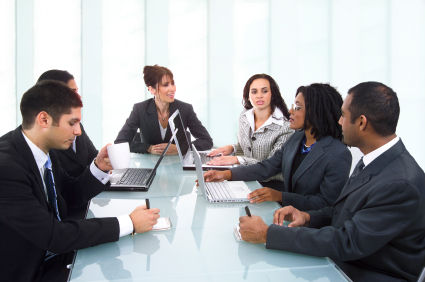
\includegraphics[width=0.8\textwidth]{img/reunion}
	\end{column}
\end{columns}
\end{frame}

\begin{frame}
\frametitle{Monitoreo y seguimiento del proyecto}
\framesubtitle{Worklogs}
\begin{itemize}
    \item Medio de comunicación pasivo.
	\item Sirve de documentación.
	\item Traspaso de conocimiento (experiencia).
	\item Verificar trabajo.
	\item Las bitácoras son siempre útiles.
\end{itemize}
\end{frame}

